\documentclass[conference]{IEEEtran}
\IEEEoverridecommandlockouts
% The preceding line is only needed to identify funding in the first footnote. If that is unneeded, please comment it out.
\usepackage{cite}
\usepackage{amsmath,amssymb,amsfonts}
\usepackage{algorithmic}
\usepackage{graphicx}
\usepackage{textcomp}
\usepackage{xcolor}
\def\BibTeX{{\rm B\kern-.05em{\sc i\kern-.025em b}\kern-.08em
    T\kern-.1667em\lower.7ex\hbox{E}\kern-.125emX}}

\usepackage{luatextra}
\usepackage{currvita}
%
\usepackage{makeidx}  % allows for indexgeneration
\usepackage{url}
\usepackage{doi}
%\usepackage[biblabel]{cite}
%\usepackage{amsmath,amssymb,amsfonts}
%\usepackage{algorithmic}
%\usepackage{graphicx}
%\usepackage[pdftex]{graphicx}
%\usepackage[dvips]{graphicx}
\usepackage{alltt}
%\usepackage{textcomp}
\usepackage{enumitem}
%\usepackage{indentfirst}

%
% Used for displaying a sample figure. If possible, figure files should
% be included in EPS format.
%
% If you use the hyperref package, please uncomment the following line
% to display URLs in blue roman font according to Springer's eBook style:
% \renewcommand\UrlFont{\color{blue}\rmfamily}


\usepackage{hyperref}
\hypersetup{
    % bookmarks=true,         % show bookmarks bar?
    unicode=true,          % non-Latin characters in Acrobat’s bookmarks
    pdftoolbar=true,        % show Acrobat’s toolbar?
    pdfmenubar=true,        % show Acrobat’s menu?
    pdffitwindow=false,     % window fit to page when opened
    pdfstartview={FitH},    % fits the width of the page to the window
    %pdftitle={},    % title
    %pdfauthor={Author},     % author
    %pdfsubject={Subject},   % subject of the document
    %pdfcreator={Creator},   % creator of the document
    %pdfproducer={Producer}, % producer of the document
    %pdfkeywords={keyword1, key2, key3}, % list of keywords
    %pdfnewwindow=true,      % links in new PDF window
    colorlinks=true,       % false: boxed links; true: colored links
    linkcolor=black,          % color of internal links (change box color with linkbordercolor)
    citecolor=black,        % color of links to bibliography
    filecolor=black,      % color of file links
    urlcolor=black,           % color of external links
    final=true
  }

\setmainfont{Times New Roman}
\renewcommand{\doitext}{DOI:}
\begin{document}

% \title{Recommender system for high school entrants having social network accounts}

\title{Two recommender systems: Technical decisions and lesson learned}

\author{%
\IEEEauthorblockN{Evgeny Cherkashin${}^{1,2}$, Viktoria Kopylova${}^2$, Boris Shevchenko${}^2$, Nikita Luk'yanov${}^2$}
\IEEEauthorblockA{${}^1$~\textit{Laboratory of Complex informational systems},\\\textit{Institute for system dynamics and control theory, SB RAS,}
Irkutsk, Russia \\
eugeneai@irnok.net}
\IEEEauthorblockA{${}^2$~\textit{Institute for informational technologies and data analysis},\\
\textit{National research Irkutsk state technical university,} Irkutsk, Russia\\
kopylovika@mail.ru, lukyanovnd@istu.edu}
}

\maketitle

\begin{abstract}
  The research of the paper is devoted to expose experience gained in development recommender systems for two domain areas: real estate of a region and choosing the specialty of a high school by entrants. These systems implement different approaches to obtain data and the technique of figuring out the user interest. The common in the techniques are the usage of preliminary data analysis for user and object classification that reduces the computations and data stored. %The recommendation is to be realized on the base of data obtained from his/her account of a social network.  Recommenter system data analysis engine is a complex of data analysis technologies being used for social network data extraction and storage, enrolling documents parsing, entrants and study subjects classifications, construction of the correlations between entrants and subjects of study.

Technique of overcoming ``cold start'' problems in these domains are proposed.  A general system design and implementation are considered.  The future development is indicated.

  % This paper deals with mostly with the stage of information acquisition, correlation patterns construction and taxonomy construction for entrants and high school subjects.
\end{abstract}

\begin{IEEEkeywords}
recommender system, taxonomy, cold start, cluster analysis, web application
\end{IEEEkeywords}

\section{Introduction}

Recommender systems (RS), being considered as an example of decision support systems, are useful to support users with additional information and decision variants.  In this paper we consider our experience with developing RS in two domains: real estate of a region and choosing the specialty of a high school.  Both systems were developed within master degree at Institute for informational technologies and data analysis, National research Irkutsk state technical university.  That's why they have status of pilot projects showing the basic technique implementations.

The first system deals with the problem of selling real estate: a flat, a room in a flat, a house.  Most of the objects on the market have similar characteristics in a class, the user interest is expressed with obvious characteristics like price, location, level, number of owners.  But the most interesting aspect of the problem is the special cases of realty like private family hotels, countryside houses, shops.  These are usually being sold for a long time, and the real estate firms utilize too many efforts for that.  The time spent to find new owner of the property is critical for the business: sellers have losses due paying the taxes for the estate being not utilized, buyers have no possibilities to invest available capital.   RS focusing user interest on the previously filtered subsets of the property, preliminary sorting by relevance, could speed up the sales.

Each school student sooner or later faces the problem of choice of a future specialty, university to enroll, and the set of courses to study.  Decisions made at this time significantly affect their future life, their job and career perspectives, families' life level.  Therefore, any help at this stage seems to be a necessary. In comparison to the real estate, where there is a whole industry supporting decision-making -- the services of realtors --, in this field the educational environment supports only an information provision service: students are given only career guidance, advertisement for the high school capabilities.  The student is on his/her own in the fundamental life decision.  Of course, parents and favorite mentors can supply the additional life experience examples helping to focus the analysis of the present conditions, but the actuality of their advices are generally of questions due to specifics of their experience, subjectivity, absence of the topical information of the present state of the labor market, scientific progress, \emph{etc}.

%[[Here we speak about actuality... how to obtain it with data analysis relating contemporary enrollments and, possibly, the resulting educational capabilities of the students after the graduation.]] [[Then transit to the preliminary part (at this time we will deal with the entrant stage) - choice of the study courses]]

% Sometimes, having received an education, people realize that they do not want to work in this area. In order to minimize the percentage of such situations, educational institutions hold various events: open days, career guidance work among school graduates, posting useful information on the websites of their university or college, \emph{etc}.  These activities help educational institutions in finding and attracting potential applicants for admission and further study in a more efficient and purposeful way.

In a period of intense competition, multidisciplinary educational institutions with similar areas of study are interested in a tool that allows them to determine the target audience more accurately, as well as entrants are interested to find a relevant university.  The work with the audience would be focused and directed. This will help to attract applicants interested in a particular direction, which is being implemented in the educational institution.  This tool could improve the effectiveness of career guidance activities for high school students.  Recommender systems are the tools of such kind.

\emph{Recommender systems} (RS) \cite{rs_basics} are decision support information systems designed to assess the user's level of interest in a particular product or service (object) based on available information about user and object.  The RS development industry began to actively develop with the emergence of online sales services, and now it is one of the active areas of development of decision support systems, a direction of artificial intelligence, focused primarily on commercial use, as well as on solving problems of increasing the productivity of searching for relevant information.

Our experience gained when producing a prototype RS for the above mentioned domains is expressed as already built and published at Github.com \cite{RSPO} RS, and in the second RS, being now on the stage of data source import routines implementation.

\section{Related works}

There are many research groups and commercial firms dealing with developing RS technologies for various domains.  We will consider related domains and other interesting cases.

In \cite{br22} a case-based reasoning RS for real estate market is presented.  Its goal is to find a similar instance in the database of existing cases, describing the cases for the user.  The obtained relations are used in following collaborative filtration and content filtering.  In theoretical research \cite{br20} the users are divided on sellers and buyers.  Sellers ``advertise'' their realty by highlighting the important features by their opinion.  So the sellers play expert roles for forming data for content filtration.  Research \cite{br23} showed that usage of Internet does not influence significantly on the time efficiency, flexibility and satisfaction criteria of the search for a flat to buy.  There are no statistical difference between 2009 and 2011, since in 2011 88\% of buyers used Internet just as the main source of information.  Authors created RS with case based reasoning utilizing an ontology model.

In \cite{br23} authors highlight three key features which significantly affects the decision: location, housing unit properties and price.  Final decision is made after evaluation of the environment, such as distances to shops, kindergartens, schools.  This can be accounted reducing the additional data to the value of the feature of housing unit properties using ontology.  The environment constraint is entered by user: user draws a circle around the preferable location, which should contain interested services and realty.

Paper \cite{br21} considers a complex logistic problem of organization of a process of real estate control, involving various people group in changing business environment.  The main aim is to develop a model, where the groups will be maximally satisfied in a rational micro and macro environment.  The efficiency of the realty utilization is evaluated with criteria of market, ownership, renewal prices, capacity, number of operations to be done while ownership transferring, safety, comfort, the time of physical and technical exploitations, \emph{etc}.  The software functions shift from ``the most economically efficient control of the property'' to multicriterial choice, raising computation efficiency.

% TODO: review of entrants' RS.

For recent RS dealing with student's problem of choice the following papers were observed. In \cite{belotsky} an RS is constructed for helping entrants to choose an education direction (expressed as sets of corresponding high schools) according to his/her grades in GCE (General certificate of education), gained competing prizes, physical activity, and hobby.  Three methods of content filtration were implemented: by distances between vector characteristics, axiomatic method of Pareto-set contraction, and analysis of hierarchies.  Authors figured out coefficients relating study directions to the features of user using series of experimental assessments controlled by experts.

In \cite{bakh}, a problem of learning outcomes assessment of higher education students is considered.  A course RS on the base students' graduate attributes, which describe their developing values, is proposed.  RS rates improvement after each course and suggests new courses by a collaborative filtering algorithm in order to improve student's average competence profile.  Students are presented as long vectors of courses they already taken with the corresponding grades.  Similarity is calculated with a variation of angle cosine of the vectors.  The recommendations are the prediction of the grades for the new courses.  Similar by the problem statement paper \cite{amer}, where RS predicts course learning trajectory patterns, the students is suggested elective curses.  Source data for collaborative filtering are existing learning trajectories acquired from senior students in the image and likeliness one student advices younger one. Students and courses are divided on clusters.  For each student cluster (a group), a mean student values are calculated.  RS algorithms are based on combination of collaborative filtering and fuzzy-like rule based system, which defines process of production of a decision.  The article has a good reviews of related works and three classical approaches basics.

Work \cite{naren} has the similar aim to develop RS for advising students new courses, but is focusing on description of courses, taking advantage of natural language processing over course documents to acquire descriptions.  Feature descriptions contain formal course data (name, structure, lecturer) and a placement in a keyword appearance frequency space.  Existing student data, represented as grades of the courses he/she already got, related to the course data.  The resulting recommendations are represented as top-5 new courses, where student will gain the best grades.  This is a simplistic direct approach and, by authors opinion, gives good results; some measurement supporting the opinion were carried on.


% frvei of paper selection.

Interesting research has been done in \cite{br10}, where the problem of overcoming the cold start problem in recommending genres and music compositions, as well as movies.  The authors developed the RS ``EZSurf'' automating the process of web surfing and content filtering using a user profile on the social network ``VKontakte'', as well as API services \texttt{last.fm} and TheMovieDB, to obtain information about similarity of the objects.  This approach greatly simplifies storage of RS data, since it does not require the designing own system of classifications.  In \cite{br14}, a problem of choosing top--$N$ objects, with higher evaluations of user interest, in content filtration.  Authors proposed RS model based on fuzzy sets, RS quality assessment technique, and a corresponding algorithm.  The models have been tested on \texttt{last.fm} data.

In a comprehensive RS review dealing with text (scientific) document relevance grading \cite{br13}, authors noted that more than half (55\%, 34 of 62) RS were based on content filtration.  Collaborative filtration was used only in 18\% (11 of 62) cases.  Stereotype based and hybrid methods are also presented.  Authors concluded that 81\% in of cases modeling user does not produce significant results in comparison to explicit indication the set of keywords.  The papers were described by keywords and, less frequently, $N$--grams included in the text, as well as metadata such as authors and references.  Most popular recommending model is based on vector space approach.  User interest modeling is implemented with graphs, where vertices are the papers, and arcs are their relationships, and topic lists assigned to user by machine learning.  The topics are organized in hierarchical catalogs using ACM classifiers.  In the RS which used collaborative filtration, the explicit ratings was not collected at all as users were too lazy to supply a rating to a paper he/she looked through.  Implicit ratings were obtained by measuring the number of pages user read, document user interaction (loading, editing), co--loadings, co-view and co-citing by users of one group.

The collaborative filtration is currently more popular as it reflects practical experience: most of RS R\&D have to solve ``cold start'' problem of initial lack of information on objects and users, as well as have adaptation to user group interest transformations due to modern trends.

% TODO: Указать, в чем особенность наших двух проектов.

Our research is aimed at application of known techniques to the objects and agents data of real estate market of Irkutsk region and, similarly, the market of education service of the region, as well as at implementation of libraries for constructing RS using nowadays technologies.

\section{Data source for RS}

\subsection{Real estate RS}

In Russian sector of Internet, real estate market is presented with various \emph{classified advertisement} websites for selling goods, jobs positions, real estate, cars, services, like \texttt{Avito.ru}.  In Irkutsk region and Moscow, every second flat is sold via such services, with publishing a number of offers for the same flat.  This usually results in reduction of the price to the level below the average on the market.  In Ekaterinburg, real estate is generally sold by realtor firms, in this case the process is more predictable for the seller.  The number of deals in Irkutsk region was raising by 20\% from 2010 to 2016 on the secondary housing market.  This increase is due to the raising of the activity of the websites.

The source of the real estate data is \texttt{atlcom.ru} that provide an actual database for real estate market of almost any region or city of Russia.  One can register and supply filter setup by a form for selection of the part of the database to download. The downloaded data are represented in XML format.  The format is developed by \texttt{Yandex.com} within the R\&D of describing selling commodities.  A special variant is for real estate.

The file comprises a list of \texttt{offer} records (subtrees) describing a flat, house or a room.  The description include metadata (where published, sale agent), location address, price, area in square meters, a photo, number of rooms, floor level, type of building and its general characteristics, as well as the conditions for obtaining additional information.  Each record is identified by a global identifier.

The RS users (agents) have roles: unknown, seller, buyer, owner, realtor, expert, and invalid user.  Before registering users' have role ``unknown'' and as each object in the system is assigned an GUID (global 128 bit identifier) related to the web browser with cookies.  With this cookie and GUID user is being tracked: the RS server collects data on his/her interest in acquiring offers identifiers being visited on the RS website.  An offer is graded as positive if user has spent more than predefined seconds viewing its webpage.  According to the review \cite{br13} forcing user to explicitly grade an offer is useless.

Users having role ``expert'' are for construction of the taxonomy of realty objects, naming of the obtained taxons (classes of realty), and storing the results in the database.  Expert's service is needed at the stage of development of the general principles of RS functioning at the cold start, the main problem we are to solve within the R\&D.  Realtor role is connected with data load activities (select a XML file, import it in the database, control the results).  In Fig. \ref{fig:use-case} we showed the Use case diagram of the system functions.

\begin{figure}[tb]
  \centering
  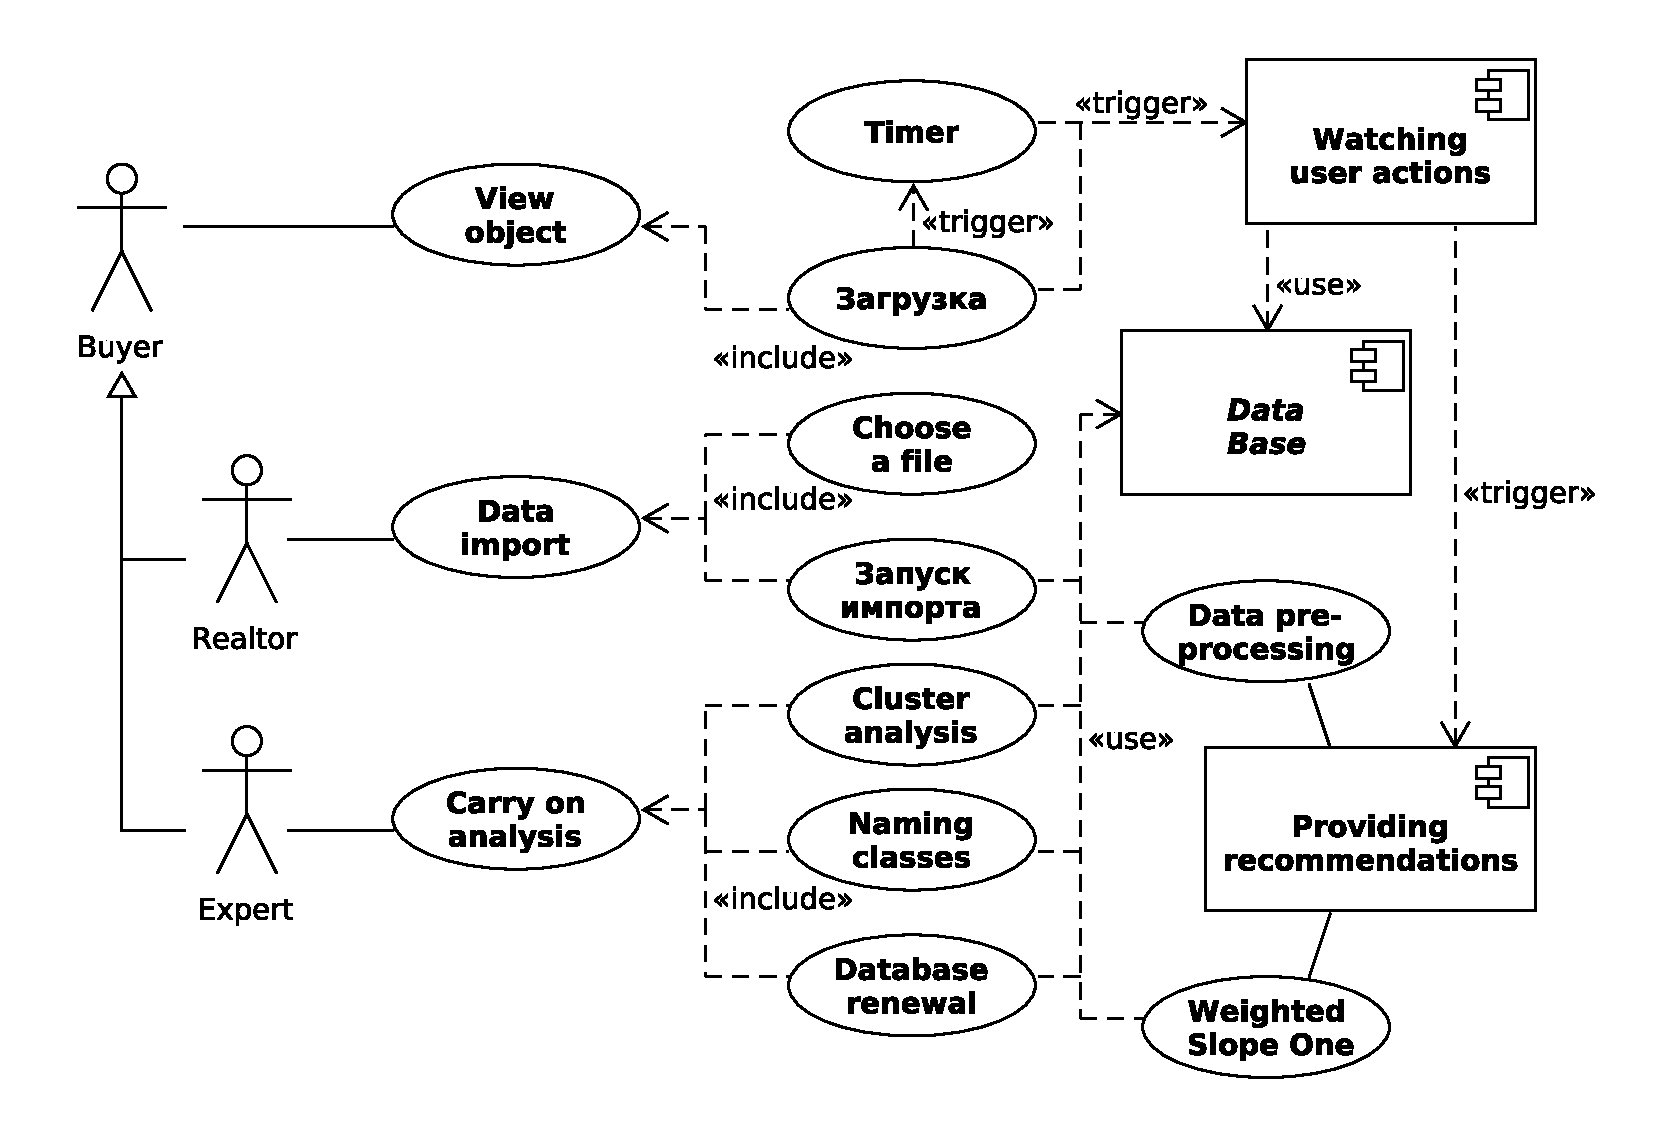
\includegraphics[width=\linewidth]{use_case.eps}
  \caption{Use case diagram for real estate RS}
  \label{fig:use-case}
\end{figure}

Therefore, the constructed RS w3as to be based on \emph{collaborative filtration} technique, where there is no expert data available for the object of user interest.  To support our case, note, that the set of offers is dynamically changed day-by-day, and it is very hard to supply the data with expert decisions reflecting all user classes opinions.  Having expert constructed the taxonomy, which seems to be made once, the new ``flats'' can be classified easily by measuring the distances to the representative instances of the classes.  The taxonomy allows us to consider the class of the realty as the object of user interest, a set of similar realty is a property characterizing the class.

\subsection{Entrants' RS}

Functioning of an RS could be based on analysis of entrants' personal properties, matching them with already enrolled students, analyzing existing individual direction of training and even a particular educational program.  We have been developing and implementing a prototype RS for helping to choose a direction of training at a university for entrants on the base of algorithms for predicting their possible choice based on digital footprints in a social network. As a source data, \emph{e.g.}, subscriptions of Russian social network ``In Contact'' (IC) (in Russian -- ``В контакте'') are used as sources of personal characteristics, and enrollment orders of our university.  %The research \cite{c1} of Tomsk state university, Russia, shows that students (pupils) once or twice a year actualize their profile and subscriptions, as irrelevant information in the main tape (blog) results in necessity to routinely filtering it out. In 2016, the university researchers showed the IC profile in general actually reflects the cognitive properties of personality, and the educational interests of students are closely correlated to their social network behavior.

Nowadays social networks are one of the main places of person's life, and even more so for a teenager.  This is clear from the data from the Glas Runet online poll service.  Among the 2000 participants of the survey, the majority (86\%) of them know about the existence of Internet social networks and use their services.  Among those who know about the existence of social networks, only 10\% do not use them \cite{c2}.
The most popular social networks according to the Romir holding are Odnoklassniki, VKontakte and Instagram.  The youngest audience, from 14 to 30 years old, visits VKontakte, 45\% does it daily, and 70\% does more often than once a day \cite{c6}.

Often, it is in social networks that one can track users' self-expression, interests and attitude to the world. The analysis of groups, posts on the main blog, reposts, statuses, \emph{etc.} can be the sources of the valuable information \cite{c7}.

Of course, if a person is an adult, then it is unlikely that all subscriptions to groups will be relevant (``entered and forgot'').  But school students, according to research \cite{c11}, update subscriptions every six months or a year: irrelevant content in the feed annoys them.  Accordingly, subscriptions can become the original dataset that can be analyzed.

In 2016, Tomsk State University researchers proved that the VKontakte profile reflects the cognitive personality traits, \emph{i.e.}, the educational interests of schoolchildren are closely related to their behavior in the social network \cite{c9}.

%Based on the data on students enrolled in various areas of a university, it is possible to build a system of recommendations for the direction of training.

\subsection{Basics of entrants' RS}

There are three basic approaches to development of an RS: \emph{content-based filtering}, \emph{collaborative filtering} and implementing as a \emph{knowledge-based system}.  Collaborative filtering is efficiently used when there is no initial data on object features describing user interests to the items, as well as definitive set of items features, which used in representing user's interest aspects.  This approach is based on continuous data accumulation of user's behavior (the decision made) within a system (\emph{e.g.}, internet shop).  In our case we cannot collect user's decision for each individual user continuously as user makes only one decision which faculty he/she will study at.

This can be done for user classes; each enrollment entrants are classified and their decisions update their classes collected data.  As this is done rarely, usually once a year, and can be processed off-line, then content-based filtering is more suitable approach for this function mode.  The third approach could be usable later after acquiring more data for data mining.

% Из Википедии - общий план исследования.

% Content-based filtering
For the ease of further consideration of the RS basic aspects of development, we took ``Content-based filtering'' section of Wikipedia webpage \cite{wikiRS}, presenting it here with a small font and necessary emphasizing, and filled it with our data, presenting with the regular font.

{\footnotesize
Content-based filtering methods are based on a description of the item (course in our case) and a profile of the user's (student and entrant in our case) preferences \cite{wb41,wb42}. These methods are best suited to situations where \emph{there is known data on an item} (name, location, description, \emph{etc.}), but \emph{not on the user}. Content-based RS treat recommendation as a \emph{user-specific classification problem} and learn a classifier for the user's preferences (likes and dislikes) based on an item's features.}

The item's source data are documents, enrollment orders, where all the formal data presented for each enrolled student.  In contradiction, we have all data about user's features from their IC profiles.  Thus, we have to design machine learning structure relating entrant's features to the classes of courses of a university.

{\footnotesize
In this system, \emph{keywords} are used to \emph{describe the items} and a \emph{user profile} is built to indicate the \emph{type of item} this user likes. In other words, these algorithms try to recommend items that are similar to those that a \emph{user liked in the past}, or is examining in the present. It does not rely on a user sign-in mechanism to generate this often temporary profile. In particular, various candidate items are compared with items previously rated by the user and the best-matching items are recommended. This approach has its roots in information retrieval and information filtering research.
}

In order to obtain the keywords describing courses, we are to create a taxonomy of courses and relate it to the known characteristics, for example, competence names or keywords obtained from course descriptions.  User profile is built out of the analysis of the user's profile and subscriptions at IC.  We cannot obtain information on the previous behavior for the individual entrants, but we can consider as a user a class of similar users, \emph{i.e.}, join users in classes and treat a class as a RC user.  New entrants are classified and their IC profiles represent new data on user's past behavior.

{\footnotesize
To create a user profile, the system mostly focuses on two types of information:
\begin{enumerate}
\item A \emph{model of the user's preference}.
\item A history of the user's interaction with the recommender system.
\end{enumerate}
}

Model of user's preference implemented as relation of user class profile features to a study course features expressed by keywords.

{\footnotesize
Basically, these methods use an item profile (i.e., a set of discrete attributes and features) characterizing the item within the system. To abstract the features of the items in the system, an item presentation algorithm is applied. A widely used algorithm is the tf–idf representation (also called vector space representation) \cite{wb43}. The system creates a content-based profile of users based on a weighted vector of item features. The weights denote the importance of each feature to the user and can be computed from individually rated content vectors using a variety of techniques. Simple approaches use the average values of the rated item vector while other sophisticated methods use machine learning techniques such as Bayesian Classifiers, cluster analysis, decision trees, and artificial neural networks in order to estimate the probability that the user is going to like the item \cite{wb44}.
}

We decided to use neural networks for the estimation, as nowadays there appeared a bunch of good programming libraries, which are easily applied.

% {\footnotesize
% A key issue with content-based filtering is whether the system is able to learn user preferences from users' actions regarding one content source and use them across other content types. When the system is limited to recommending content of the same type as the user is already using, the value from the recommendation system is significantly less than when other content types from other services can be recommended. For example, recommending news articles based on browsing of news is useful, but would be much more useful when music, videos, products, discussions etc. from different services can be recommended based on news browsing. To overcome this, most content-based recommender systems now use some form of hybrid system.
% }

% {\footnotesize
% Content-based recommender systems can also include opinion-based recommender systems. In some cases, users are allowed to leave text review or feedback on the items. These user-generated texts are implicit data for the recommender system because they are potentially rich resource of both feature/aspects of the item, and users' evaluation/sentiment to the item. Features extracted from the user-generated reviews are improved meta-data of items, because as they also reflect aspects of the item like meta-data, extracted features are widely concerned by the users. Sentiments extracted from the reviews can be seen as users' rating scores on the corresponding features. Popular approaches of opinion-based recommender system utilize various techniques including text mining, information retrieval, sentiment analysis (see also Multimodal sentiment analysis) and deep learning \cite{wb45}.
% }

In general, the research consists of our variant of the standard scenario that includes the following steps:
\begin{enumerate}
\item Import and analyze enrollment orders existing at the university administration;
\item Crawl the social network for personal characteristics and subscriptions for all student included in the enrollment orders;
\item Import curriculum data for all courses we interested in, gathering related data such as competence;
\item Creating taxonomies for students and study courses, name resulting classes, juxtapose them with related data;
\item Devising classification procedures for relating entrants to the classes;
\item Imported and above mentioned data analysis results organized in a rational database having wrapped in an ORM (Object-relational mapping) to ease of usage;
\item Implementation the content-based filtering for students that are entrants with data in the database.
\item Create web application for entrants and university staff.
\item Testing the system and interviewing students.
\end{enumerate}

There are regular problems of feature selection describing users and study courses, as well as naming their classes after stage of taxonomy inference.  The subscription group (channel) names can be used as features too.  They also could be processed with clustering to generalize subsets of groups, giving additional data on the similarities and control correspondence to their set of subject tags.  As for names of courses classes competence names can be used also possibly after a generalization.  Classification of new students is to be implemented with two-layer neural network for easy implementation. The data will be processed in context of the university and its subdivision departments, institutions.  There is other data that could be used in the preliminary data analysis: faculty name, course relation data, competence definition text, relation of competences to their courses, course data like study direction and other describing features, and, in principle, results of feed text analysis.




% Смотри. В этом разделе надо показать, как актуализировать текущее состояние рынка образовательных услуг и рынка профессий для абитуриента. И. Как для университету сделать так, чтобы он мог, например, в ленту конкретного школьника подсовывать свою рекламу (целевая аудитория).

% Но такая реклама это же таргетированная... И это раздел СММ вроде бы...

% Я думала это программа типа помощь с тем, чтобы выбрать направление обучения

% Для реализации проекта необходимо выполнить следующие задачи:
% - осуществить постановку задачи и описать требования к системе;
% - получить набор данных (синтаксический анализ открытых приказов о поступлении);
% - разработать алгоритм поиска студентов в социальной сети «Вконтакте» (ВК) при использовании технологии API;
% - спроектировать и реализовать базу данных (БД);
% - разработать основные классы, выполняющие взаимодействие пользователя с БД и обработку поступающих данных;
% - реализовать графический интерфейс;
% - осуществить тестирование и отладку программы;
% - разделить данные на обучающую и тестовую выборку;
% - подобрать и реализовать алгоритм классификации данных, наиболее подходящий для достижения поставленной цели;
% - обучить алгоритм и проверить на тестовой выборке;
% - протестировать алгоритм на данных о поступивших в следующем году абитуриентах.

\section{Technologies used}
\label{sec:tech}

In both projects we used C\#-based platform \cite{ben16} for implementation as it is a compromise of expressiveness and computational performance, it has rich set of libraries and frameworks.  The RS are web ASP.NET and MONO applications with database represented with Entity Framework Object-relational mappers (ORM) \cite{ef15}.  One of the advantages of the C\# language is partial classes allowing composition of a class dividing its definition between files, which can be both generated and programmed manually.  This technology supports great flexibility of Entity Framework.  The language also supports properties and decorators, making it a convenient application programming language.

Database back-end of the realty RS is open-source RDF (Resource Description Framework) triple store \texttt{BrightstarDB}, allowing in future research to use data in logical inference engines, \emph{e.g.}, for constructing knowledge-based RS and connect the system with other servers via SPARQL.  The second RS back-end database is SQLEXPRESS, the default setup for Microsoft Visual Development Studio.

The input data for entrants' RS is provided by the input forms and automatic processing of students enrollment orders in DOCX format, using our syntactic analyzer.  Orders contain header, which is parsed to determine the date of the enrollment, specialty and other parameters.  The only table part lists of the enrolled students.  Additionally, the list records are checked by regular expressions determining the sum of points gained.  The reading of the document data is implemented by means of C\# library \texttt{Microsoft.Office.Interop.Word} with its \texttt{Paragraphs} collection and \texttt{Range} objects.

The list of students is traversed, and for each student his/her IC profile is queried.  The data of interest are the profile and the subscriptions.  The query is done via IC API as HTTP queries \cite{apivk}.  According to IC API policy, the queries can be issued not more than three times per second, otherwise error 6 meaning ``Too many requests per second'' is obtained.  Additional constraints are stated to the set of issued remote methods.  The policy for the set is not published, its violation results to the Captcha test issue or rejection of a concrete method usage with no restriction for others.

% The database is used to query stored data

One student can have more than one IC accounts.  In this case a form appeared to choose the right one manually.  The decision is stored in a database table attribute.

% Curriculum structure is analyzed by a Python script.  It loads Excel spreadsheet containing the working plans for a student group and extracts disciplines, working hours, competences and various formal data from there.  The structure is stored in a database.

\section{Preliminary data processing}
\label{sec:relim-proc}


%\subsection{Input data acquisition}
%\label{sec:tech-input}

% The acquired input data stored in the database at first is processed with hierarchical cluster analysis algorithms to construct set of classes for students and study courses.  After that, a classification procedure is applied to construct relations between individual student to its class.  These classifications allow us to reduce the complexity of the main recommender algorithms and shift partially from collaborative filtration technique to ....

In realty RS, two program agents are implemented, which are executed on an event occurrence.  The first one starts by timer of web browser and implements issuing user positive evaluation, if user spends some time viewing a page of a realty object.  The second one, located at the server side, is activated if the first one raised event of a positive evaluation.  Server agent receives the evaluation and may start recalculation of estimates for recommendations if there are enough computational resources.

All data are stored in a database, which structure is represented as objects in Figure~\ref{fig:class-siag}.  Central entity is \texttt{IOffer}, representing the offer of a realty object.  The information on an object, which is independent of an offer, is stored as \texttt{IObject}-object.  The object structure corresponds to standard Yandex and Google form of real estate representation.

\begin{figure*}[tb]
  \centering
   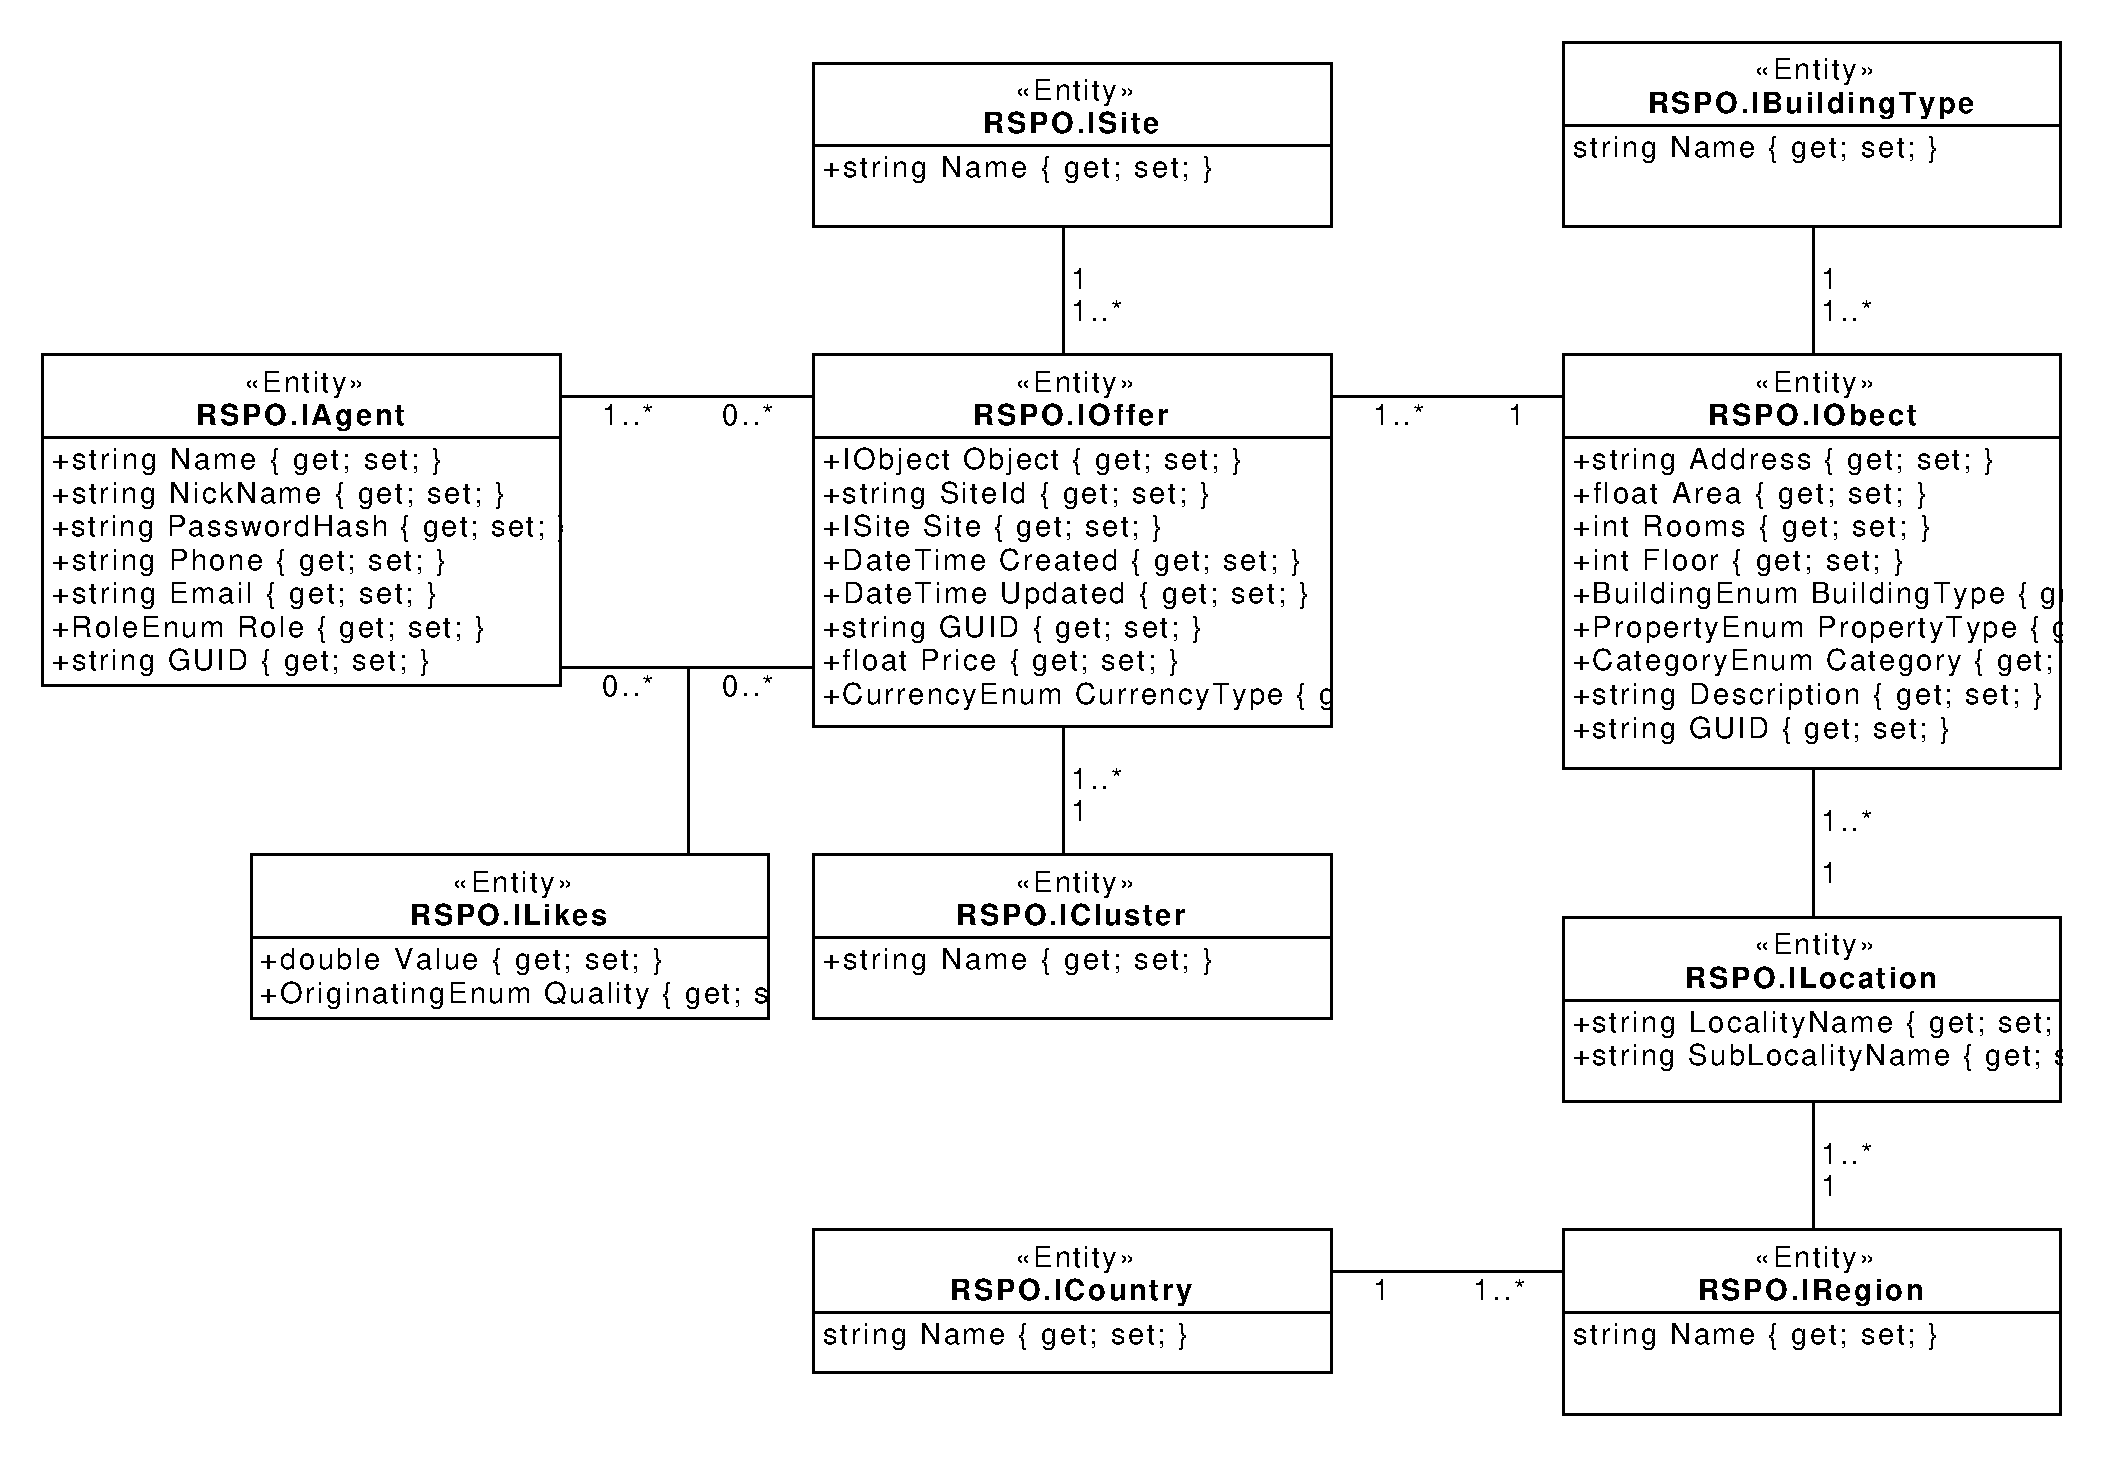
\includegraphics[width=0.7\linewidth]{class_diagram.pdf}
  \caption{Class diagram for real estate RS}
  \label{fig:class-siag}
\end{figure*}

The real estate domain specifics is the total availability of data for realty objects, so the import function provides the whole body of information on objects by importing it from other sites.


\subsection{Classification of realty objects}
\label{sec:class-realty}

% The classification was carried out with hierarchical clustering method and c\# library ....

Comparison of the object is done in a vector space according to the features presented in Table~\ref{tab:cmp}.
\begin{table}[tb]
  \caption{Comparing features and their weight coefficients}
  \label{tab:cmp}
  \footnotesize
  \centering
  \begin{tabular}{|l|l|c|c|}
    \hline
    Attribute & Calculation technique & $v_k, \%$ & Formula \\
    \hline
\texttt{string Name} & not used & & \\
    \texttt{ILocation Location} & equality & 10 & $(\star)$
    \\
\texttt{string Address} & --''-- & 10 & \\
\texttt{float Price} & relative difference & 25 & $(\star\star)$\\
\texttt{CurrencyEnum \ldots} & not used  & & \\
\texttt{float Area} & relative difference  & 35 & $(\star\star)$\\
\texttt{AreaUnits AreaUnit} & not used & &\\
\texttt{string ImageURL} & --''-- & & \\
\texttt{string URL} & --''-- & & \\
\texttt{int Rooms}  & relative difference  & 100 & $(\star\star)$\\
\texttt{int RoomsOffered} &  --''--   & 100 & $(\star\star)$\\
\texttt{int Floor}  &  --''--   & 30 & $(\star\star)$\\
\texttt{int FloorTotal}  &  --''--   & 10 & $(\star\star)$\\
\texttt{BuildingEnum \ldots}  & equality & 30 & $(\star)$\\
\texttt{IBuilding \ldots{}}  & --''-- & 30 &  $(\star)$\\
\texttt{PropertyEnum \ldots} & --''-- & 30 &  $(\star)$\\
\texttt{CategoryEnum \ldots} & --''-- & 100 &  $(\star)$\\
\texttt{string Description} & not used & & \\
    \texttt{string GUID} & --''-- & & \\
    \hline
  \end{tabular}
\end{table}

In the table with stars we denote the following formulas:
\[
  d_k(i,j) = \left\{
                                                          \begin{array}{ll}
                                                            0, & \mbox{if\ \ } a_i=a_j,\\
                                                            1, & \mbox{if\ \ } a_i\neq a_j,
                                                          \end{array}
                                                          \right.
  \tag{\star}
\]
\[
  d_k(i,j) = \frac{|a_i^k-a_j^k|}{a_i^k+a_j^k},\quad a_i^k+a_j^k>0.
  \tag{\star\star}
\]

The aggregate assessment is made with formula:
\[
  d(i,j)=\frac{\sum\limits_{k=1}^m|v_k\cdot d_k(i,j)|}{\sum\limits_{k=1}^m v_k}, \qquad 0\leqslant d_{i,j}\leqslant 1,
\]
\noindent where $v_k$ is a weight of $k$-th attribute value, defined in the table. %, we, as programmers, for each calculated $d(i,j)$ \texttt{asserted} its value $0\leqslant d(j,j)\leqslant 1$.

In order to create a taxonomy, expert user must run the hierarchical clustering function supplying the number $N$ of general clusters to figure out.  After the function finishes, expert will see the numbers of top $N$ clusters with number of their objects.  Next step is naming the clusters.  Expert enters the subsets and reviews the objects, forming an image of the common properties of the objects.  After naming the image in the first interface, expert changes name of cluster from a number to the name.  This is to be done for each $\overline{0,N-1}$ cluster.  If expert cannot form a concrete image of the class, them we recommend repeat the procedure with larger number of clusters.

Some clusters can gain the same name, and after renaming, clusters with the same name are joined.  Hierarchical clustering allows us to make experiments with data without recalculation of the taxonomies.  Before running clustering function, expert can restrict the set of objects to be examined, \emph{e.g.} by 200 objects, so we can use even agglomerative hierarchical clustering.

The following classes are presented on Irkutsk region real estate market: two-room flats, one-or-two-room flats (comfort class realty), one-room flats, dachas, houses, rooms, commercial space, a garage, and elite realty (flats with three and more rooms).

User interests are acquired as follows.  New user is suggested a set of objects from all the classes of realty.  Watching users activities, which objects he/she is viewing, the systems gains initial interest, and then specifies the class of objects to view at following steps.  Each object observed by user during long time considered to be of interest, the positive evaluation is added to database.  Recommended objects are shown in a list located at the bottom of the interface window.  The set of suggested objects is restricted by 20 items.

\section{Recommendations generation behavior}
\label{sec:proc-recs}

The RS for real estate market is implemented Slope One based collaborative filtration \cite{br1}.  We assume that buyer purchases a flat not frequently and then each buyer is a new user, and no data about his/her preferences are available, as well as one flat cannot be bought several times as compared to a regular internet shop of commodities.  New users are assigned a GUID and tracked by cookies.  Tracking data forms preference data.  After a predefined number of viewed pages, RS suggests registering, it is an engine preventing losing the data due to moving user to another workstation, and starts to issue recommendations.  The user is not required to register, as it was specially stated before us as a requirement, but we explain the advantages of the registration action.

RS tracks user movement around various classes and fixed for each class the estimation of the object explicitly viewed by user. For each visited class, RS performs filtering the set of objects and range them according to all collected user data in the context of the class.  The relevance is calculated by Slope One technique.  The average values of differences of objects' evaluations are calculated by request and cashed in the user session data. After calculation of the evaluations for each object, which was not seen by user, in the class, objects are sorted by relevance and a predefined number of them are displayed.

The Slope One algorithm can generate recommendations for an object (a class) if there is at least one positive evaluation of an object of the class.  At the cold start period if there were no such evaluations, RS shows random 20 objects of the same class of objects user is viewing.

\section{Web applications}

Both RS use MVC \cite{friman15,cchadvik20} architecture in construction of user interface.  Realty RS is based on \texttt{Nancy} ASP.NET framework, where for each URL template a lambda function is related, having supported parameters of the Request objects.  At the beginning of each function we restore \texttt{session} object, and at the end, the Response object is created by applying a context model and a view object to a template.  As template engine SharpTAL is used, an implementation of Zope page template (ZPT) with Template attribute language (TAL).  This implementation follows traditions of C\#, namely, compile its content into objects at the phase of project compilation.

As for each web template engine, ZPT uses \texttt{model}, \texttt{view}, which implements \emph{controller} functions as well, and \texttt{template} to generate HTML content.  Model is referred as \texttt{context} of a view, which function is simplification of the access to context by template, and transforming user actions into model change upon \texttt{POST} query.  For using global application and other data, as context we pass in a general case \texttt{application}, \texttt{appview}, \texttt{user} and \texttt{message} objects.  User defines the currently authenticated user, and message contains text to show in a view, announcing an event happening in the RS, \emph{e.g.} the fact that the record is successfully stored in the database.

ZPT and TAL technologies were chosen as they give a very powerful tool for HTML tree structure manipulation including usage of named and parametrized macros, attributes subtrees, defined in one-page template, and multiply used in other ones, as well as the technology tries not to extend XHTML syntax with new entities for implementation of element replacement functions.

\section{Discussion}
\label{sec:disc}

The realty RS was tested by a number of human being fictitious buyers, none of them mentioned misbehavior of the system like spontaneous transitions from one class to another, or supplying empty sets of recommendations.

The overview of the presented experience shows that C\# .NET and MONO technologies and used techniques are well suitable for construction RS of various kind, fulfilling the following typical requirements:
\begin{enumerate}
\item working in ``cold start'' conditions;
\item do not require user to register and authorize while implicit gathering information needed for recommendation generation;
\item testing systems are to be done in a local conditions to be able to check the results comparing with existing ``natural'' data;
\item using open-source technologies, modules and libraries.
\end{enumerate}

The obtained real estate RS implementation as well as the second project do not take advantage of the nowadays methods of R\&D development, which corresponds to current traditions.  Most attention is paid to preliminary data processing and obtaining minimal valuable product (MVP).

\section*{Conclusion}
\label{sec:conc}

We presented results of two master degree projects in the field of recommender system (RS) development in real estate and university entrants' study direction decision-making.  The first one is finished, and the second one is on a half way.  Both systems have similar design, but rely on different RS technique: the realty RS is based on collaborative filtration, the entrants' one is based on content filtering.  Both systems use object-oriented representation of application entities, which are persistent as well.

Solutions of ``cold start'' problem for both domains has been considered.  They are based on creating taxonomies of objects by cluster analysis and partial transition to consider classes as objects of users' interests.  In the entrant RS we also created taxonomies of users according their subscriptions in a social network.

The RS are implemented as MVC web applications for users, the administrative and expert user interfaces are implemented as window applications in entrant RS.  This simplifies user role model: web users must register, administrator runs form application at workstation and is not required to register.  Testing the finalized RS showed stable work when used by human users.

The described technique could be developed further by adaptation the standard directions such as:
\begin{itemize}
  \item development or adaptation of ontology of domain to extend search capabilities especially in students' courses domain;
  \item case based reasoning for the same domain;
  \item predictive modeling of attribute values for realty;
  \item providing geospacial data of infrastructural service organizations in the environment, \emph{e.g.} schools, kindergartens and shops.
\end{itemize}

\section*{Acknowledgements}
\label{sec:ack}

Authors thank Evgeny Vasil'evich Brezheshov, director of a realtor office, for helping with problem domain description and problem statement for real estate RS.

% \section*{References}

\begin{thebibliography}{99}
\bibitem{rs_basics} D. Jannach, M. Zanker, A. Felfernig, G. Friedrich. Recommender Systems: An Introduction. Cambridge University Press, 2010.
\bibitem{RSPO}E.~Charkashin, B.~Shevchenko. Source code of a prototype real estate market recommender system.  URL:\url{https://github.com/eugeneai/RSPO-CSharp}. (access date: 21-09-2020)
\bibitem{br22}E. M. Alrawhani, H. Basirona, Z. Sa’ayaa. Real estate recommender system using case-based reasoning approach. Journal of
Telecommunication, Electronic and Computer Engineering (JTEC).
Vol. 8 No. 2. p. 177-182.
\bibitem{br20} E.~V.~Britina. Segmenting recommender system with client--server connection based on programmable configured networks and usage protocol with fast-jumping IP-address.  // Sovremennye problemy nauki i obrazovaniya. No 6. 2015.
URL:\url{https://www.science-education.ru/ru/article/view?id=16875} (in Russian)
\bibitem{br23} X. Yuan, J.-H. Lee, S.-J. Kim, Y.-H. Kim. Toward a user-oriented recommendation system for real estate websites. Information Systems, 38 (2013). p. 231–243.
\bibitem{br21}T. Ginevičius, A. Kaklauskas, P. Kazokaitis, J. Alchimovienė.
Recommender system for real estate management. Verslas: Teorija ir
praktika (Business: Theory and Practice). 2011 12(3). p. 258–267 \doi{10.3846/btp.2011.26}
\bibitem{belotsky} E. A. Belotskiy, A. V. Suetin, Сonstruction of a recommendersystem for choosing higher education institutions for entrants, Vestnik S.-Petersburg Univ. Ser. 10. Prikl. Mat. Inform. Prots.Upr., 2016, Issue 1, 66–77. URL:\url{http://www.mathnet.ru/links/1c01f91d57c8dc6f050c7e6d3fed3604/vspui277.pdf}(in Russian)
\bibitem{bakh}B. Bakhshinategh, G. Spanakis, O. Zaiane, S. ElAtia. A Course Recommender System based on Graduating Attributes. In Proceedings of the 9th International Conference on Computer Supported Education, Volume 1: CSEDU, ISBN 978-989-758-239-4, 2017, pp. 347-354. \doi{10.5220/0006318803470354}
\bibitem{amer}A. Al-Badarenah, J. Alsakran. An Automated Recommender System for Course Selection” International Journal of Advanced Computer Science and Applications(ijacsa), 7(3), 2016. \doi{10.14569/IJACSA.2016.070323}
\bibitem{naren}J. Naren, M. Z. Banu, S. Lohavani. Recommendation System for Students’Course Selection. A. K. Somani et al. (eds.), Smart Systems and IoT: Innovationsin Computing, Smart Innovation, Systems and Technologies 141. 2020. pp.~825--833. \doi{10.1007/978-981-13-8406-6_77}
\bibitem{br10} B.~R.~Avhadeev, L.~I.~Voronova, E.~P.~Ohapkina. Development of recommender system on the base of profile in social network ``VKontakte''. Vestnik Nizhnevartovskogo gosudarstvennogo universiteta. Issue No 3. 2014. (in Russian)
\bibitem{br14}A.~S.~Amel'kin, D.~M.~Ponizovkin. Mathematical model of top-N problem for content recommender systems. Izvestiya MGTU ``MAMI'' No 3(17), 2013, Vol.2. p. 26-31. (in Russian)
\bibitem{br13} J. Beel, B. Gripp, S. Langer, C. Breitinger. Research-paper recommender systems: a literature survey // International Journal on Digital Libraries (2016) 17: 305. \doi{10.1007/s00799-015-0156-0}
\bibitem{c2}S.P.~Balandina, M.V.~Bautin, A.V.~Maiyorov, E.R.~Smirnova. Social networks as means of education and educational participants interactions. Pedagogicheskie i informacionniye tehnologii v obraxovanii. No. 15 (2016). (in Russian) URL:\url{https://journals.susu.ru/pit-edu/issue/view/31}
\bibitem{c6}K.S.~Veber, A.A.~Pimenova. Comparative analysis of social networks. Vestnik Tambovskogo universiteta. Series: Natural and technical sciences. Vol. 19, No. 2, 2014. p. 636--643. (in Russian)
\bibitem{c7}A.V.~Rozhkova. Self-expression (self-presentation) in social Internet networks as a phenomenon of human cyber-socialization. Homo Cyberus. 2017. No. 2(3). (in Russian) URL:\url{http://journal.homocyberus.ru/Samovyrazhenie_v_socialnyh_internet-setjah_kak_fenomen_kibersocializacii}
\bibitem{c11} A.V. Fescshenko. Social networks in education: experience analysis and development perspectives. Gumanitarnaya informatika, Tomsk, Issue 6. 2012. p. 124--134. (in Russian)
\bibitem{c9}V.V.~Matsuta, P.B. Kiselyev, A.V. Fescshenko, V.L. Goyko. Investigation of social networks potential for revealing talented students. Psychologiya i psihotehnika. No. 4. 2017. p. 104--121. (in Russian)
\bibitem{wikiRS}Recommender system -- Wikipedia. URL:~\url{https://en.wikipedia.org/wiki/Recommender_system} (access date: 13.09.2020)
\bibitem{wb41}Ch.C. Aggarwal Recommender Systems: The Textbook. Springer. 2016. ISBN 9783319296579.
\bibitem{wb42}P. Brusilovsky. The Adaptive Web. 2007. p. 325. ISBN 978-3-540-72078-2.
\bibitem{wb43}D.H. Wang, Y.C. Liang, D.Xu, X.Y. Feng, R.C. Guan. "A content-based recommender system for computer science publications", Knowledge-Based Systems. 2018. 157: 1-9
\bibitem{wb44}S. Blanda. Online Recommender Systems – How Does a Website Know What I Want?. American Mathematical Society. 2015.
%\bibitem{wb45}X.Y. Feng, H. Zhang, Y.J. Ren, P.H. Shang, Y. Zhu, Y.C. Liang, R.C. Guan, D. Xu, The Deep Learning–Based Recommender System “Pubmender” for Choosing a Biomedical Publication Venue: Development and Validation Study, Journal of Medical Internet Research, 2019. 21 (5): e12957
\bibitem{ben16} J.~Albahari, B.~Albahari. C\#~6.0 in a Nutshell: The Definitive Reference 6th Edition, 2015. 1138~p. ISBN-13: 978-1491927069
\bibitem{ef15}Entity Framework Tutorial. URL:\url{https://www.entityframeworktutorial.net/} (дата обращения: 05.07.2020).
\bibitem{apivk}VKontakte API documentation. URL: \url{https://vk.com/dev/manuals} (access date: 05.07.2020).
\bibitem{br1} D. Lemire, A. Maclachlan. Slope One Predictors for Online Rating-Based Collaborative. URL:~\url{http://cogprints.org/4031/1/lemiremaclachlan_sdm05.pdf} (access date: 10.05.2018)
\bibitem{friman15}A.~Freeman. Pro ASP.NET MVC 5. 5th ed. Apress. 2013. 832 p. \doi{10.1007/978-1-4302-6530-6}
\bibitem{cchadvik20} J. Chadwick, T. Snyder, H. Panda. Programming ASP.NET MVC 4: Developing Real-World Web Applications with ASP.NET MVC.  O'Reilly Media; 1st Edition. 2012. 492 p.  ISBN-13:~978-1449320317
\end{thebibliography}
\end{document}

%%% Local Variables:
%%% mode: latex
%%% TeX-master: t
%%% End:


-------------------
Reviewer #1 Comments

The papers topic is interesting and well presented, based on two separate researches.

It contributes to the conference and should be considered for further publication.

--------------------
Reviewer #2 Comments

Clear paper, but:

Introduction is too big, almost 2 full pages.

Check fonts at page 4

Please use numbers (not “*” ) for mark all formulas

In Reference list, sources form Wikipedia [19] are not suitable
